\documentclass[../report.tex]{subfiles}

\begin{document}

\chapter{\writingNotes{Use case}} \label{cha:use_case}

This chapter show a practical use case of using the newly implemented KHAPE library and the demonstrate the security benefits.

\section{Context}

\subsection{Online password manager}
Online password manager are among the most sensitive site out there because the compromise of user's data cascade into numerous account compromisation on other services such as email account, social media, banking, etc.

Using an asymmetric PAKE for an online password manager make a lot of sense because the client doesn't have to disclose it's master password to the password manager host. In other words, the client doesn't have to trust the password manager host to not decrypt its personal data and/or leak the master password (or any other intentional or unintentional miss-handling).

In fact multiple well known online password manager such as iCloud Key Vault or 1Password use aPAKE (SRP).

\subsection{Other use case}

More generally, using an aPAKE makes a lot of sense on application where the server-side stored user's data shouldn't be visible to the server (server doesn't process the data, online backup, online wallet?, secure vault, password manager, etc.). This is archived with encryption and so require an encryption key for the client.
Depending on the client, it is not feasable to store an additional symmetric key because it has to be securely stored (see HSM) which cause problem of portability and key recovery. For example, for an online encrypted backup of a laptop or smartphone, if the user loose its device, he cannot retrieve his online backup because the encryption key is stored on its lost device.

For portability, the encryption key is typically derived from the user's password --- the same password that he uses to authenticate with the server (you could require that the user input two differents passwords but this is generally avoided because of bad user experience). Using a classical authentication method, the server store the user's encrypted sensible data AND also process the password in cleartext which is used to compute the encryption key. This void all the security of encrypting the sensitive data in the first place because the server --- or an malicious party who compromised the server --- could store the cleartext password, compute the encryption key and decrypt the sensitive user's data.

This is the reason why aPAKEs are very interesting in these case senario. The server NEVER see the user's password so he cannot use it to decrypt user's data.



% How to decrypt data (password manager's data) ?
% - password in KDF
% - using initial OPRF output
% - compute a new OPRF (different salt, same password ?)



% - Context/Introduction
% - Design
%   - Encrypted envelope (khape export key)
%   - Download/upload (khape session key)
%   - Auth/Register (no password leak)
%   - User's fonctionalities (CRUD)







% \section{Design}
% - multi user online password manager
% - Server store client's encrypted password registry
% - KHAPE export key is used to decrypt password registry
%     - derived from the hardened (slowhash) OPRF output
%         - an attacker that obtained the encrypted password registry and want to bruteforce the password has to request the server for every try since he doesn't know the server's secret salt.
% - Take full advantage of KHAPE, no password leakage, use export key
% - user talk to client, client talk to server







% What is it ? what can be done, what can it be used for
% usefulness of KHAPE -> no password leakage, export key
% encrypted registry and key derivation
% server endpoints
% client action (interaction)
% limitation / considerations

\section{Online password manager implementation}

This section describe the design and the implementation of the use case: a multi-user online password manager.

The basic principle is that the server stores clients' encrypted password registry. 
Each client can only access his personal encrypted password registry and 

- multi user online password manager
- user talk to client, client talk to server
- OPRF and slowhash

% - perform double encryption
% - master key is not derived, it is encrypted
- a bit inspired by bitwarden

- authentication token, expire after 24h
- can use totp


- taken from a project 
- Currently the client is only CLI but planned to be compiled to wasm to be integrated to a browser
- Server network is simulated.
- Database



\subsection{Encrypted user data}
Each user store his encrypted user data on the server. This data include a Encrypted password registry and a Encrypted master key.


The Encrypted password registry is a structure that contains the user's password. Password are double encrypted. The external structure --- the password registry --- is encrypted and then each individual password are also encrypted. Each encryption is performed with a different key, all derived from the master key.

The Encrypted master key is simply a key --- the Master key --- that is encrypted with another key --- the KHAPE's export key. 
One could derive the Master key from the KHAPE's export key but this means that if the user want to change his authentication password, it is necessary to decrypt and re-encrypt every single password entry and the password registry with the new export key. This is not envisageable for a scalable password manager. Instead, in case of change in the authentication password, only the Master key is re-encrypted with the new export key.


ProtectedRegistry:
- ciphertext
- nonce

Registry:
- vec<PasswordEntry>
- nonce

PasswordEntry:
- label
- username
- ProtectePassword

ProtectedPassword:
- ciphertext
- nonce

Password:
- data
- nonce


\subsection{General process}

The figure \ref{fig:Online_password_manager} shows the entire process of reading a protected password from the authentication request to the password decryption.

\begin{enumerate}
 \item The user input his password in the client and the KHAPE authentication start :
 \begin{enumerate}
  \item The client
 \end{enumerate}
 \item The client finish the KHAPE authentication with a session key and an export key. The session key is verified with the server. If the inputted password is invalid, no session key is outputted. An export key would still be outputted since it is not verifiable.
 \item Client request to download its encrypted data from the server using the session key as an authentication token. The server also store the session key and can verify that the client has been successfully authenticated. An authentication token expire after 24h hours.
 \item If the authentication token is valid, the client receive his Encrypted master key and his Encrypted password registry.
 \item He decrypt the Encrypted master key with the KHAPE's export key to obtain his private key
 \item He compute two HKDF Expand with the Master key as an input and constant labels to obtain an External encryption key and an Internal encryption key
 \item He decrypt the Encrypted password registry with the External encryption key to obtain the Indexable password registry
 \item Now that the client has decrypted the external layer of the password registry, he remove the following value from memory: Export key, Master key, Encrypted master key and Encrypted password registry. He still has to keep the Session key to communicate with the server and the external encryption key to re-encrypt the password registry upon modification.
 \item In the Indexable password registry each entry's label and username is in cleartext but the password is still unreadable. 
 \item When the user choose to read a password entry, the client use Internal encryption key to compute an HKDF Expand with the entry's label and username as context. The result is a key that is unique for this password.
 \item The client finish by decrypting the encrypted password with the computed key. He obtain the readable password.
 \item After sending the cleartext password to the user, the client remove it from memory as well as the Individual password key.
\end{enumerate}

At "rest", the client keeps Session key, External encryption key, Internal encryption key and Indexable password registry

Upload:
When the client add, update or remove a password, he needs to update his Encrypted password registry and upload it to the server. This is done by computing an Individual password key from the Internal encryption key and the password entry's label and encrypting the password with this key. Then the password entry is added or updated in the password registry which is then encrypted with the External encryption key. The resulting ciphertext is sent to the server



\begin{figure}[h]
 \centering

 \setlength{\fboxsep}{10pt}
 \setlength{\fboxrule}{1pt}
 \fbox{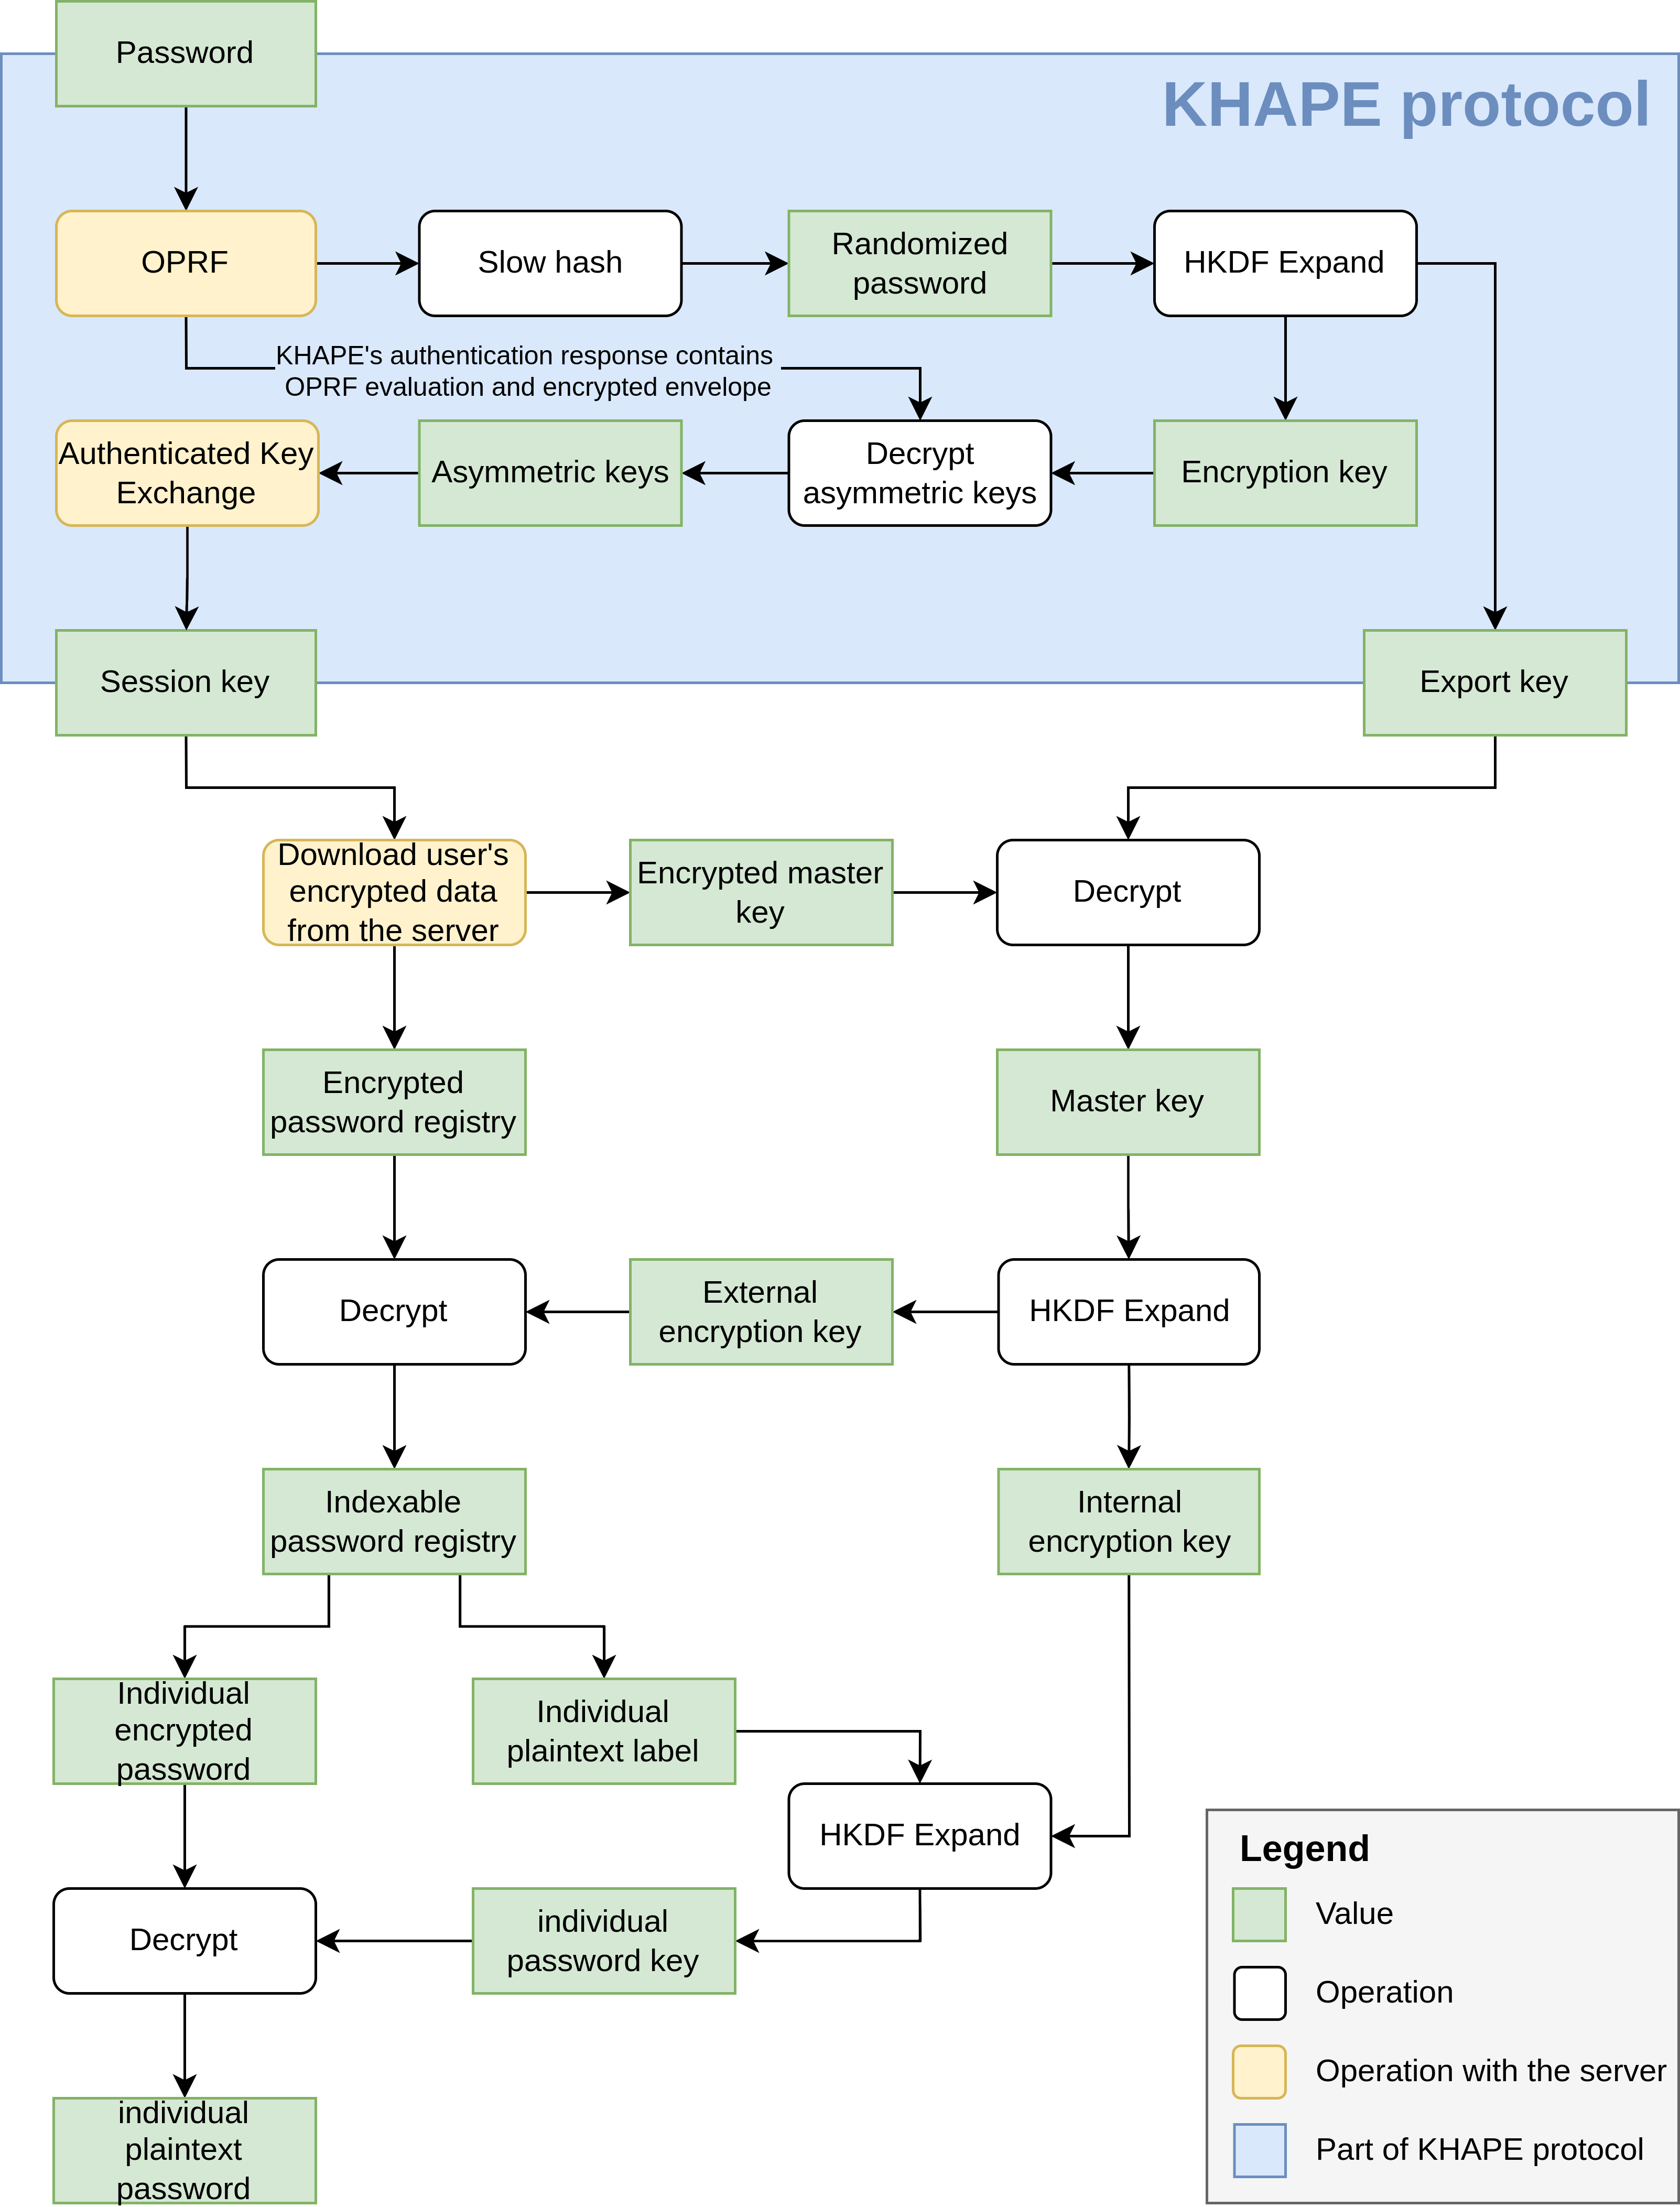
\includegraphics[width=\textwidth-22pt]{key-management.png}}

 \caption{Online password manager key derivation process to read a password.}
 \label{fig:Online_password_manager}
\end{figure}



\subsection{Server endpoints}
The server has only four endpoints:

\begin{itemize}
 \item Registration (KHAPE)
 \item Authentication (KHAPE)
 \item File download
 \item File upload
\end{itemize}

Registration and authentication are handled by KHAPE's protocol (see Section \ref{sec:khape_generic_algo}).

File download and file upload allow the user to retrieve and commit his protected data from the server. The interactions between the client and the server are defined in figure \ref{fig:usecase_download} for the file download endpoint and in figure \ref{fig:usecase_upload} for the file upload endpoint




\begin{figure}[h]
 \centering

 \setlength{\fboxsep}{10pt}
 \setlength{\fboxrule}{1pt}
 \fbox{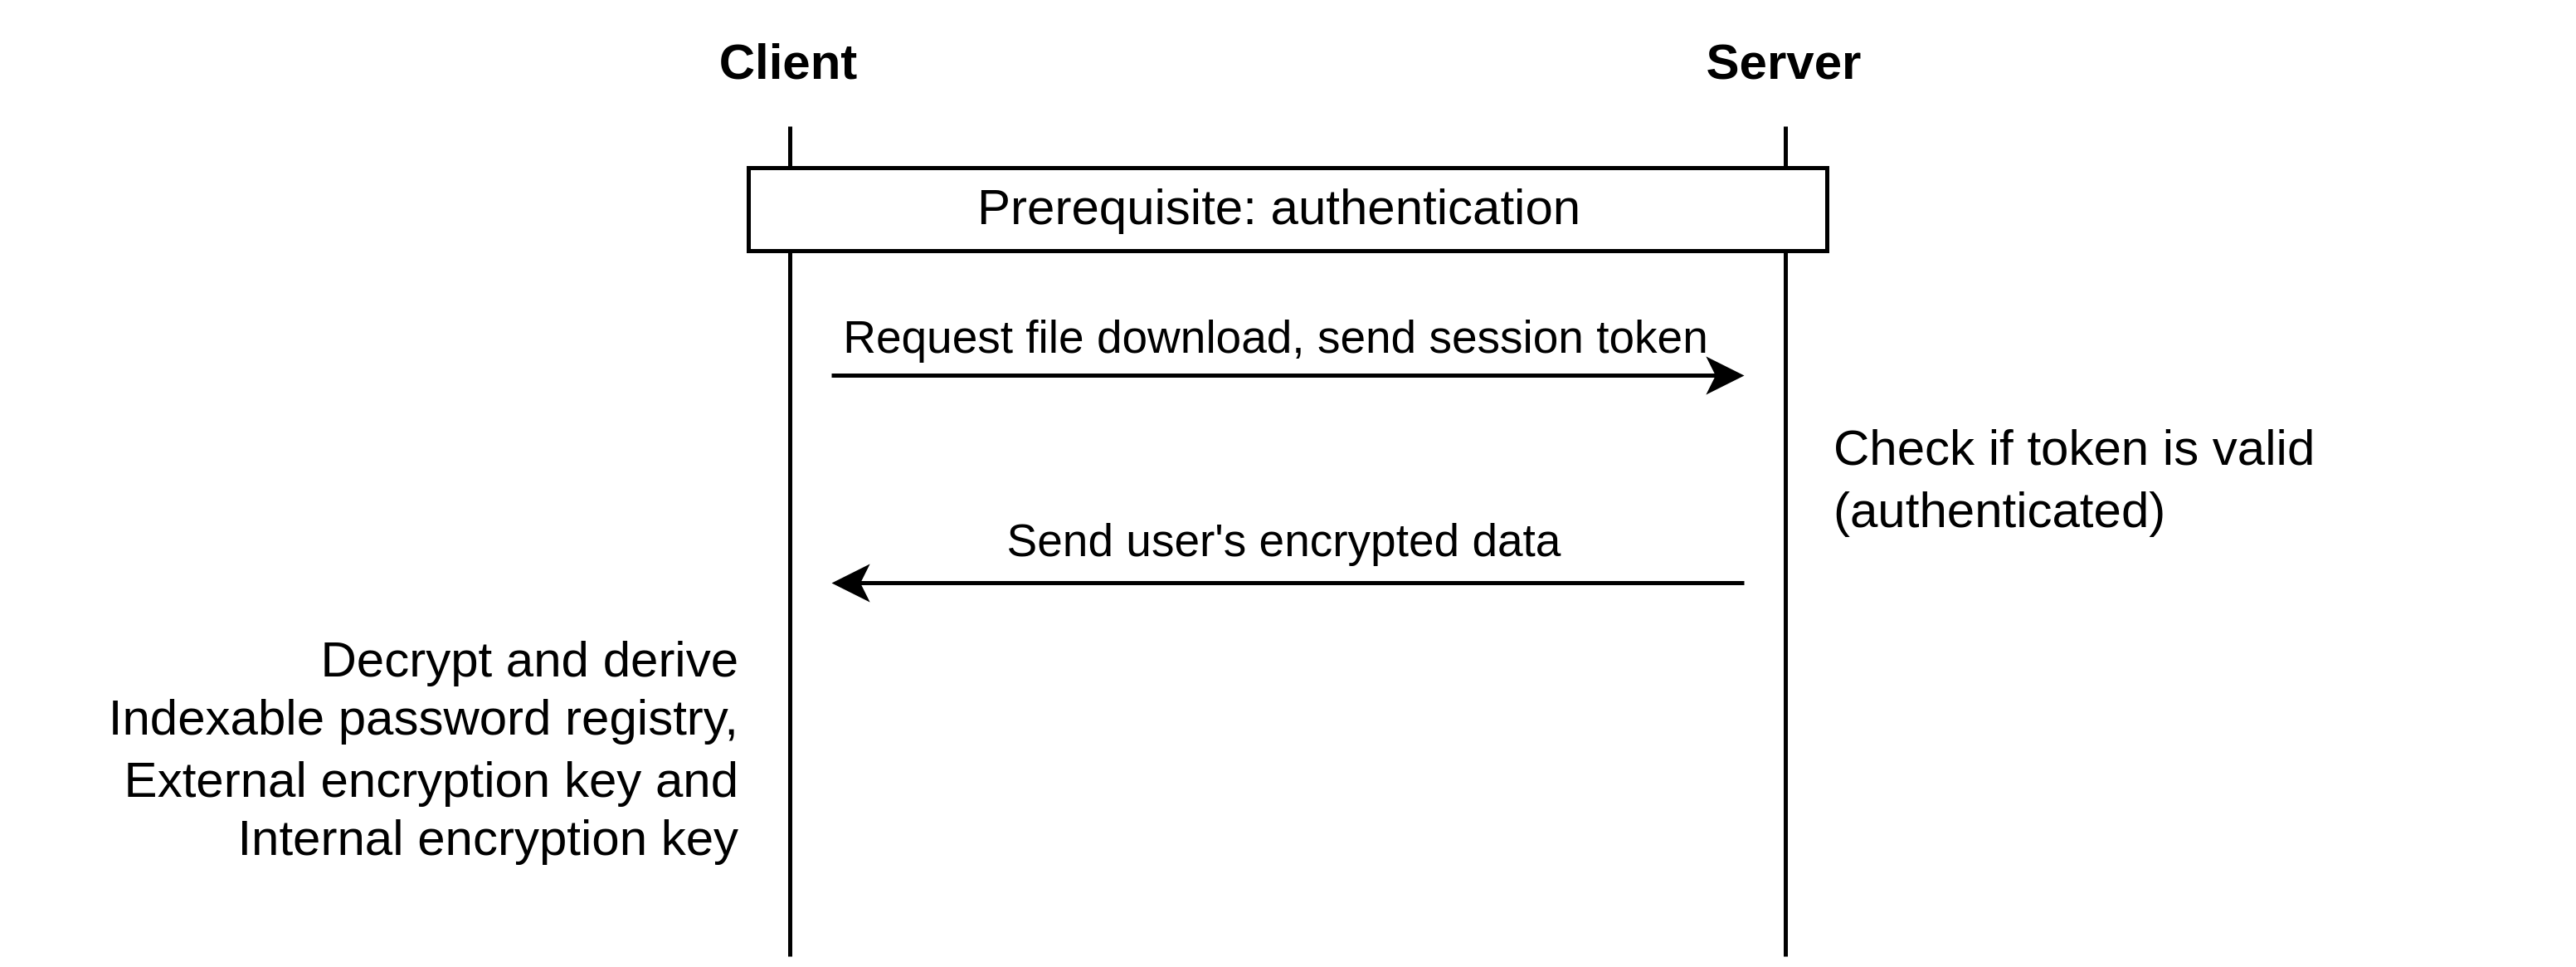
\includegraphics[width=\textwidth-22pt]{download.png}}

 \caption{Interaction between the client and the server for the file download endpoint.}
 \label{fig:usecase_download}
\end{figure}


\begin{figure}[h]
 \centering

 \setlength{\fboxsep}{10pt}
 \setlength{\fboxrule}{1pt}
 \fbox{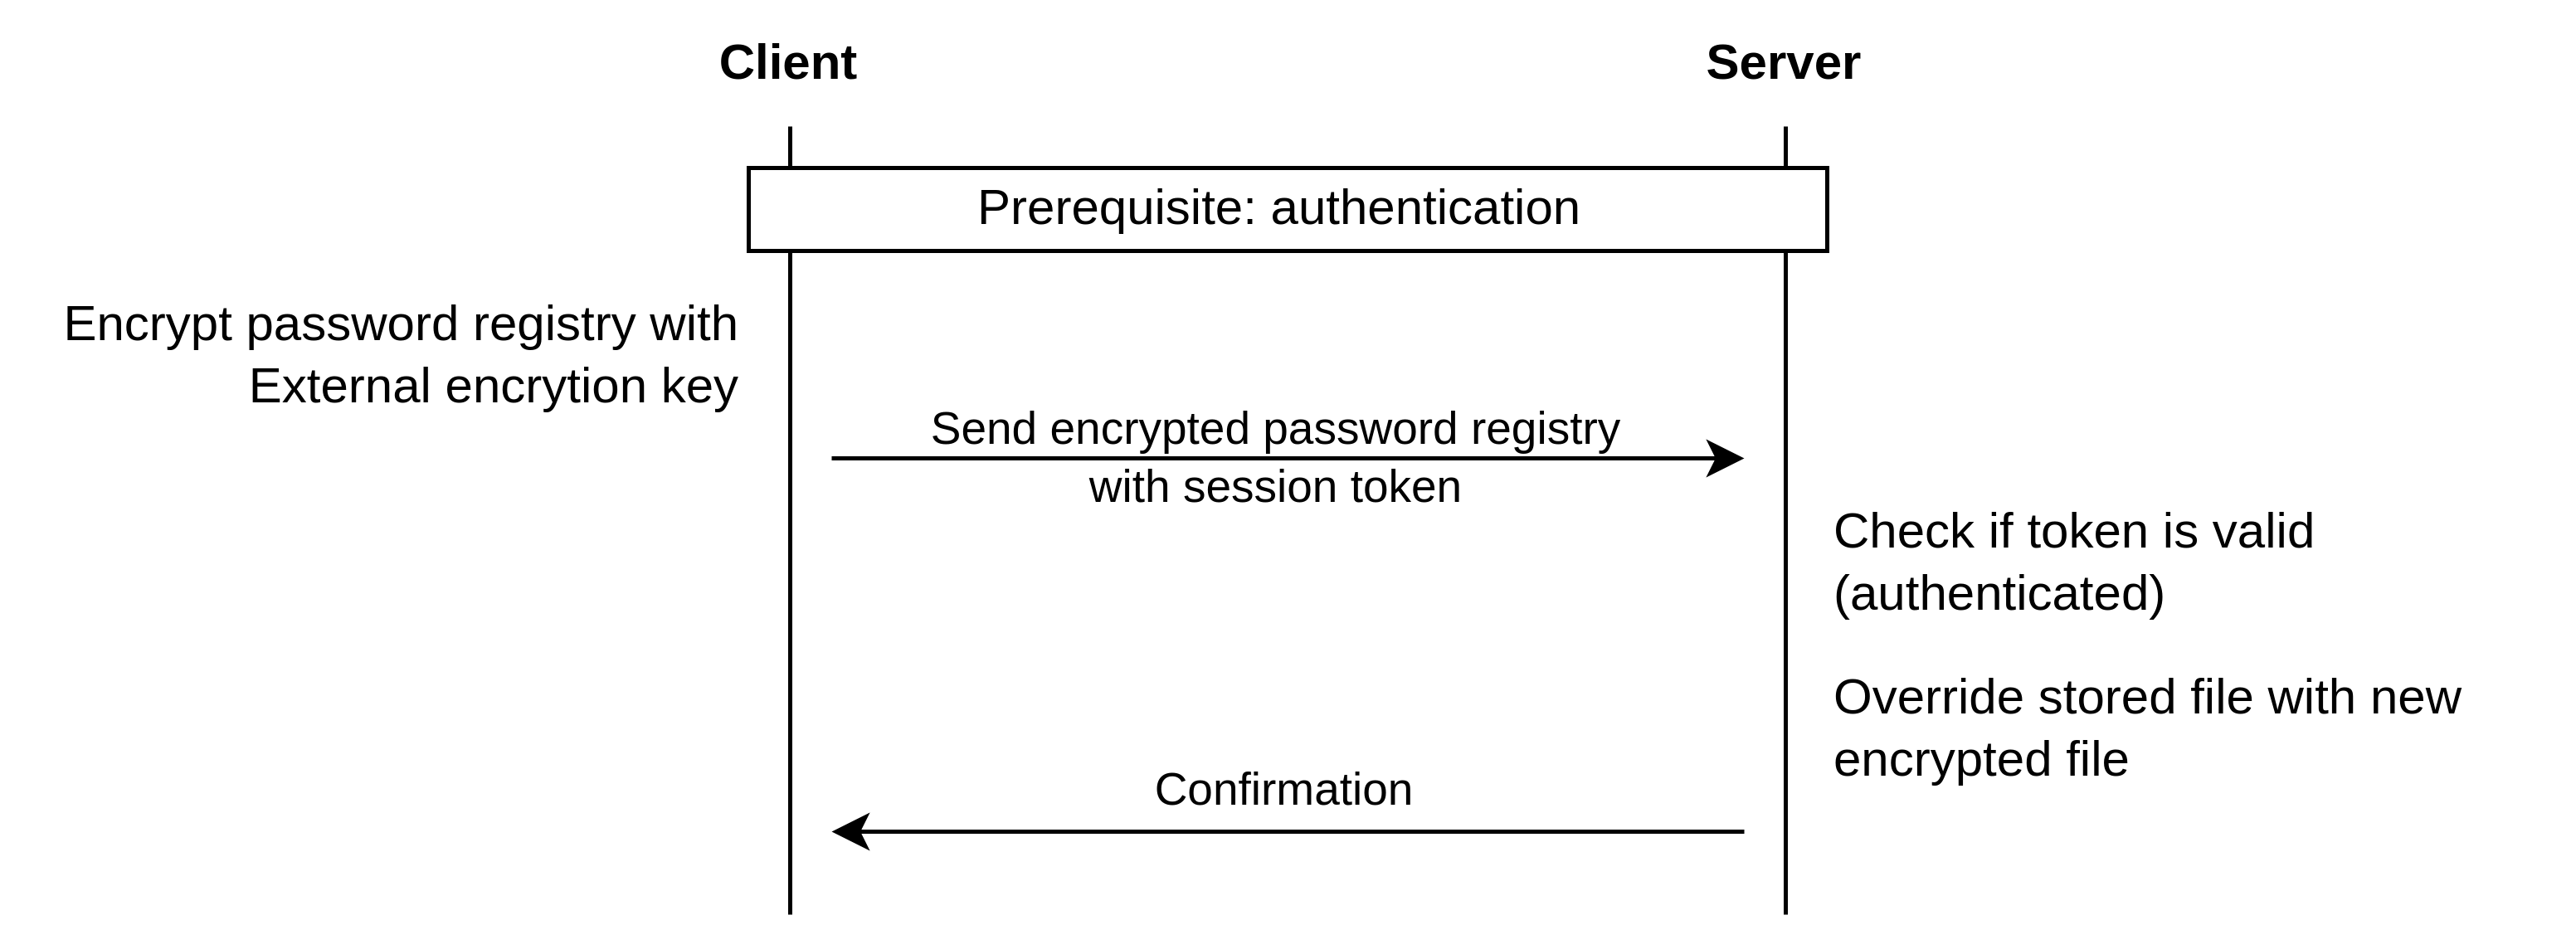
\includegraphics[width=\textwidth-22pt]{upload.png}}

 \caption{Interaction between the client and the server for the file upload endpoint.}
 \label{fig:usecase_upload}
\end{figure}




\subsection{Client actions}
The end user interact with the client to access its passwords.
At client start, the user can either register or login.
After a successful registration, he still needs to login.

Upon successful authentication, the client automatically download the user's data file and the user can select one of the following actions :

\begin{itemize}
 \item Read a password
 \item Add a new password
 \item Modify a password
 \item Delete a password
\end{itemize}

For actions where the password registry is modified (adding, modifying or deleting a password), the password registry is re-encrypted by the client (with the External encryption key) and uploaded to the server.


The interactions between the user and the client are defined in figure \ref{fig:usecase_read} for reading a password entry, in figure \ref{fig:usecase_add} for adding a new password entry, in figure \ref{fig:usecase_modify} for adding a modifying an existing password entry and in figure \ref{fig:usecase_delete} for deleting a password entry.






\begin{figure}[h]
 \centering

 \setlength{\fboxsep}{10pt}
 \setlength{\fboxrule}{1pt}
 \fbox{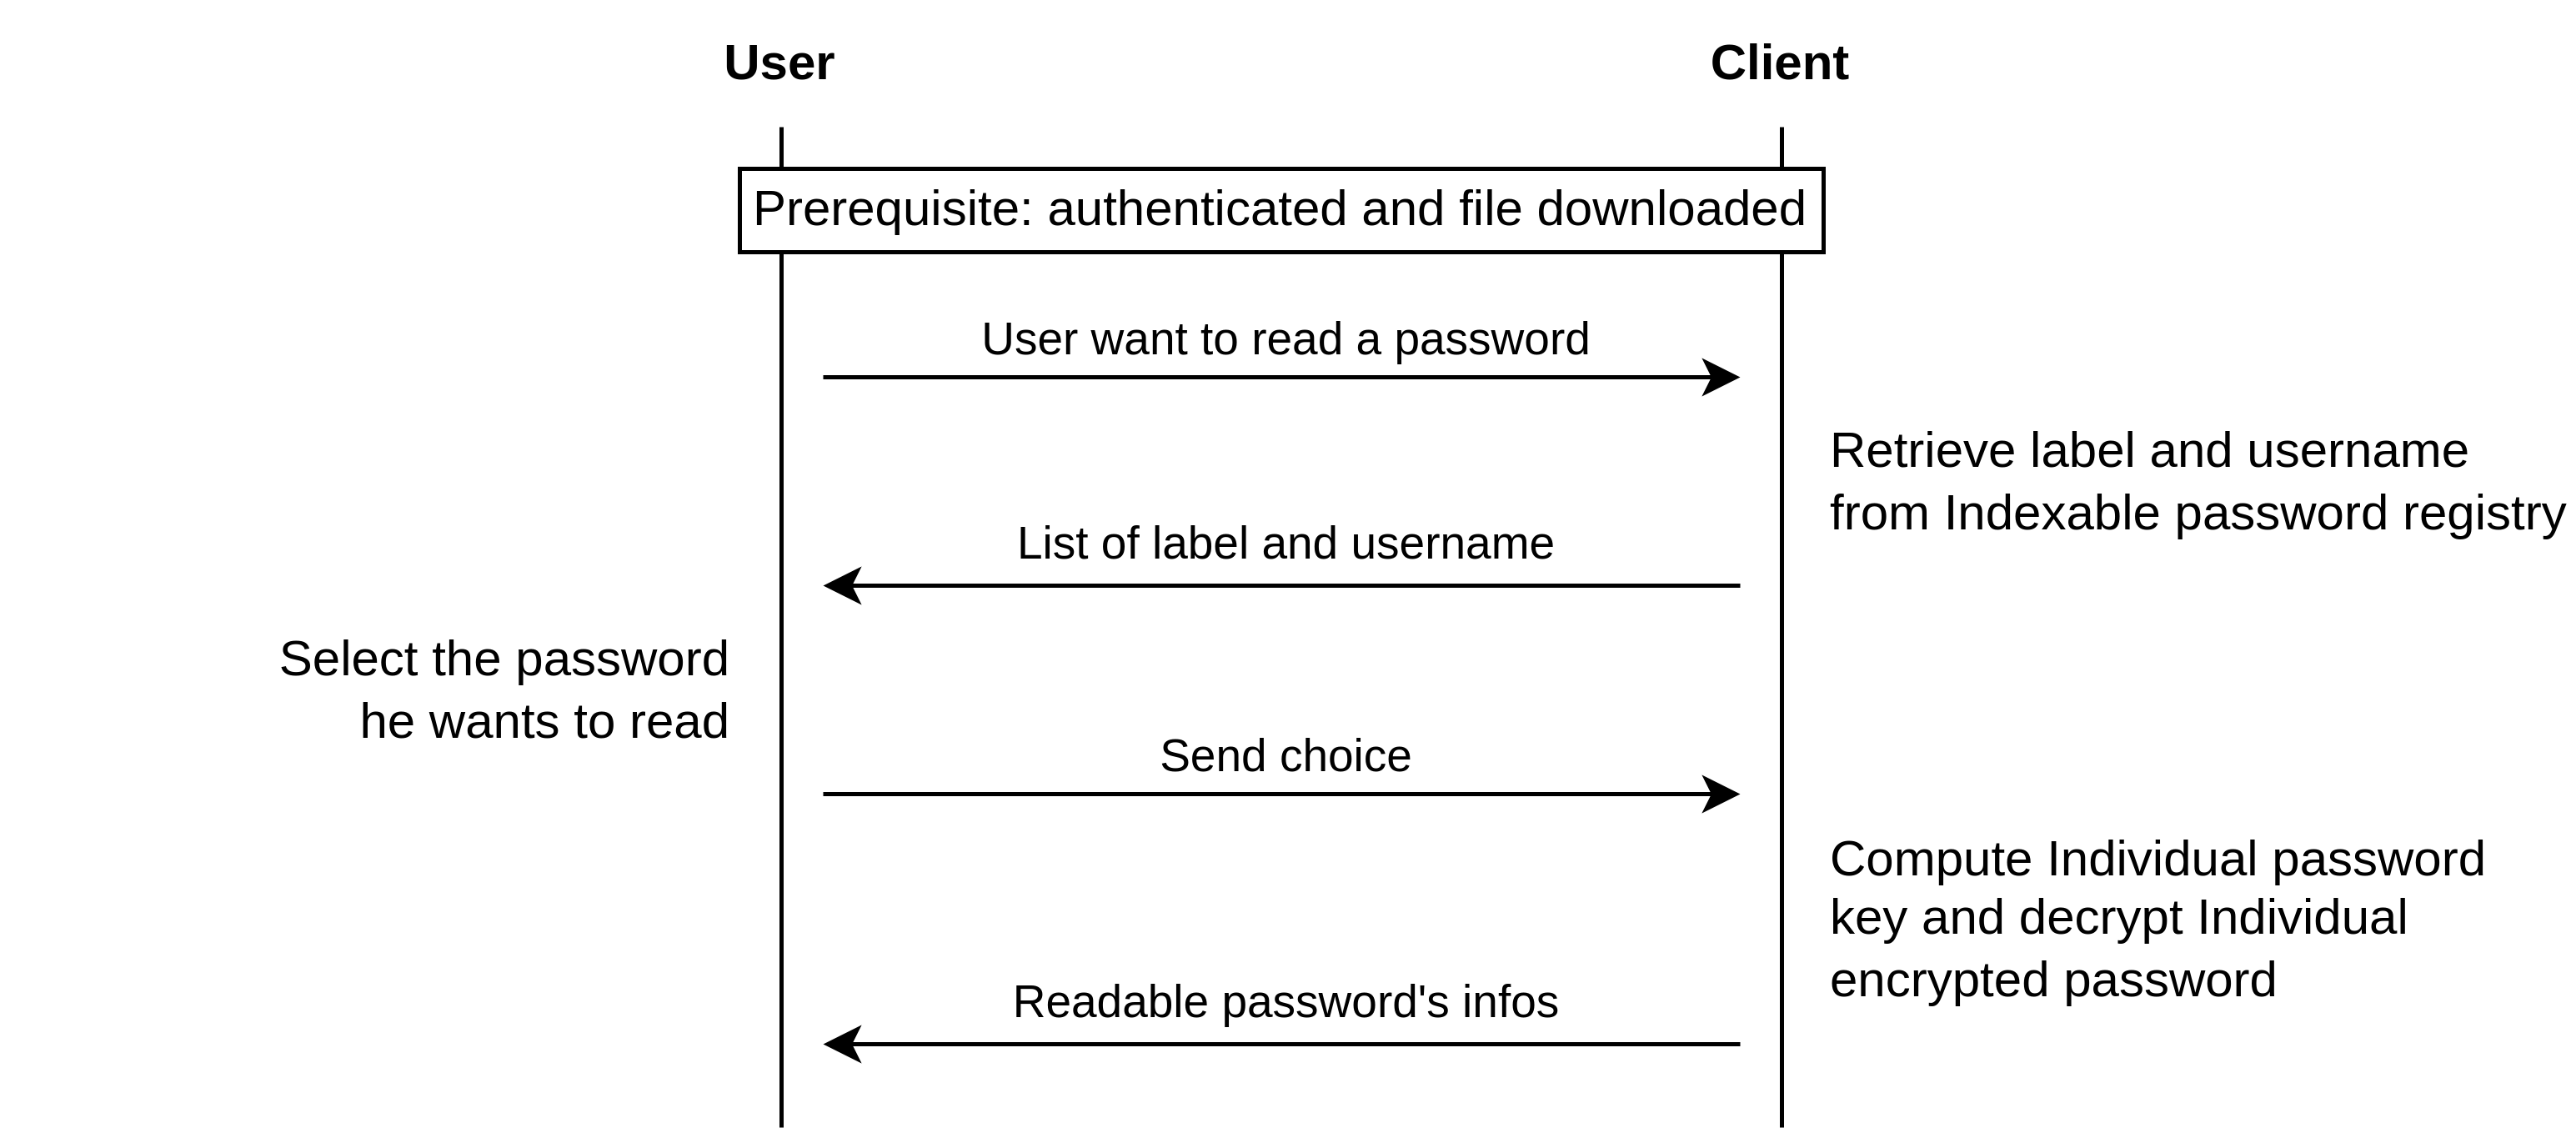
\includegraphics[width=\textwidth-22pt]{read.png}}

 \caption{Interaction between the user and the client for reading a password entry.}
 \label{fig:usecase_read}
\end{figure}



\begin{figure}[h]
 \centering

 \setlength{\fboxsep}{10pt}
 \setlength{\fboxrule}{1pt}
 \fbox{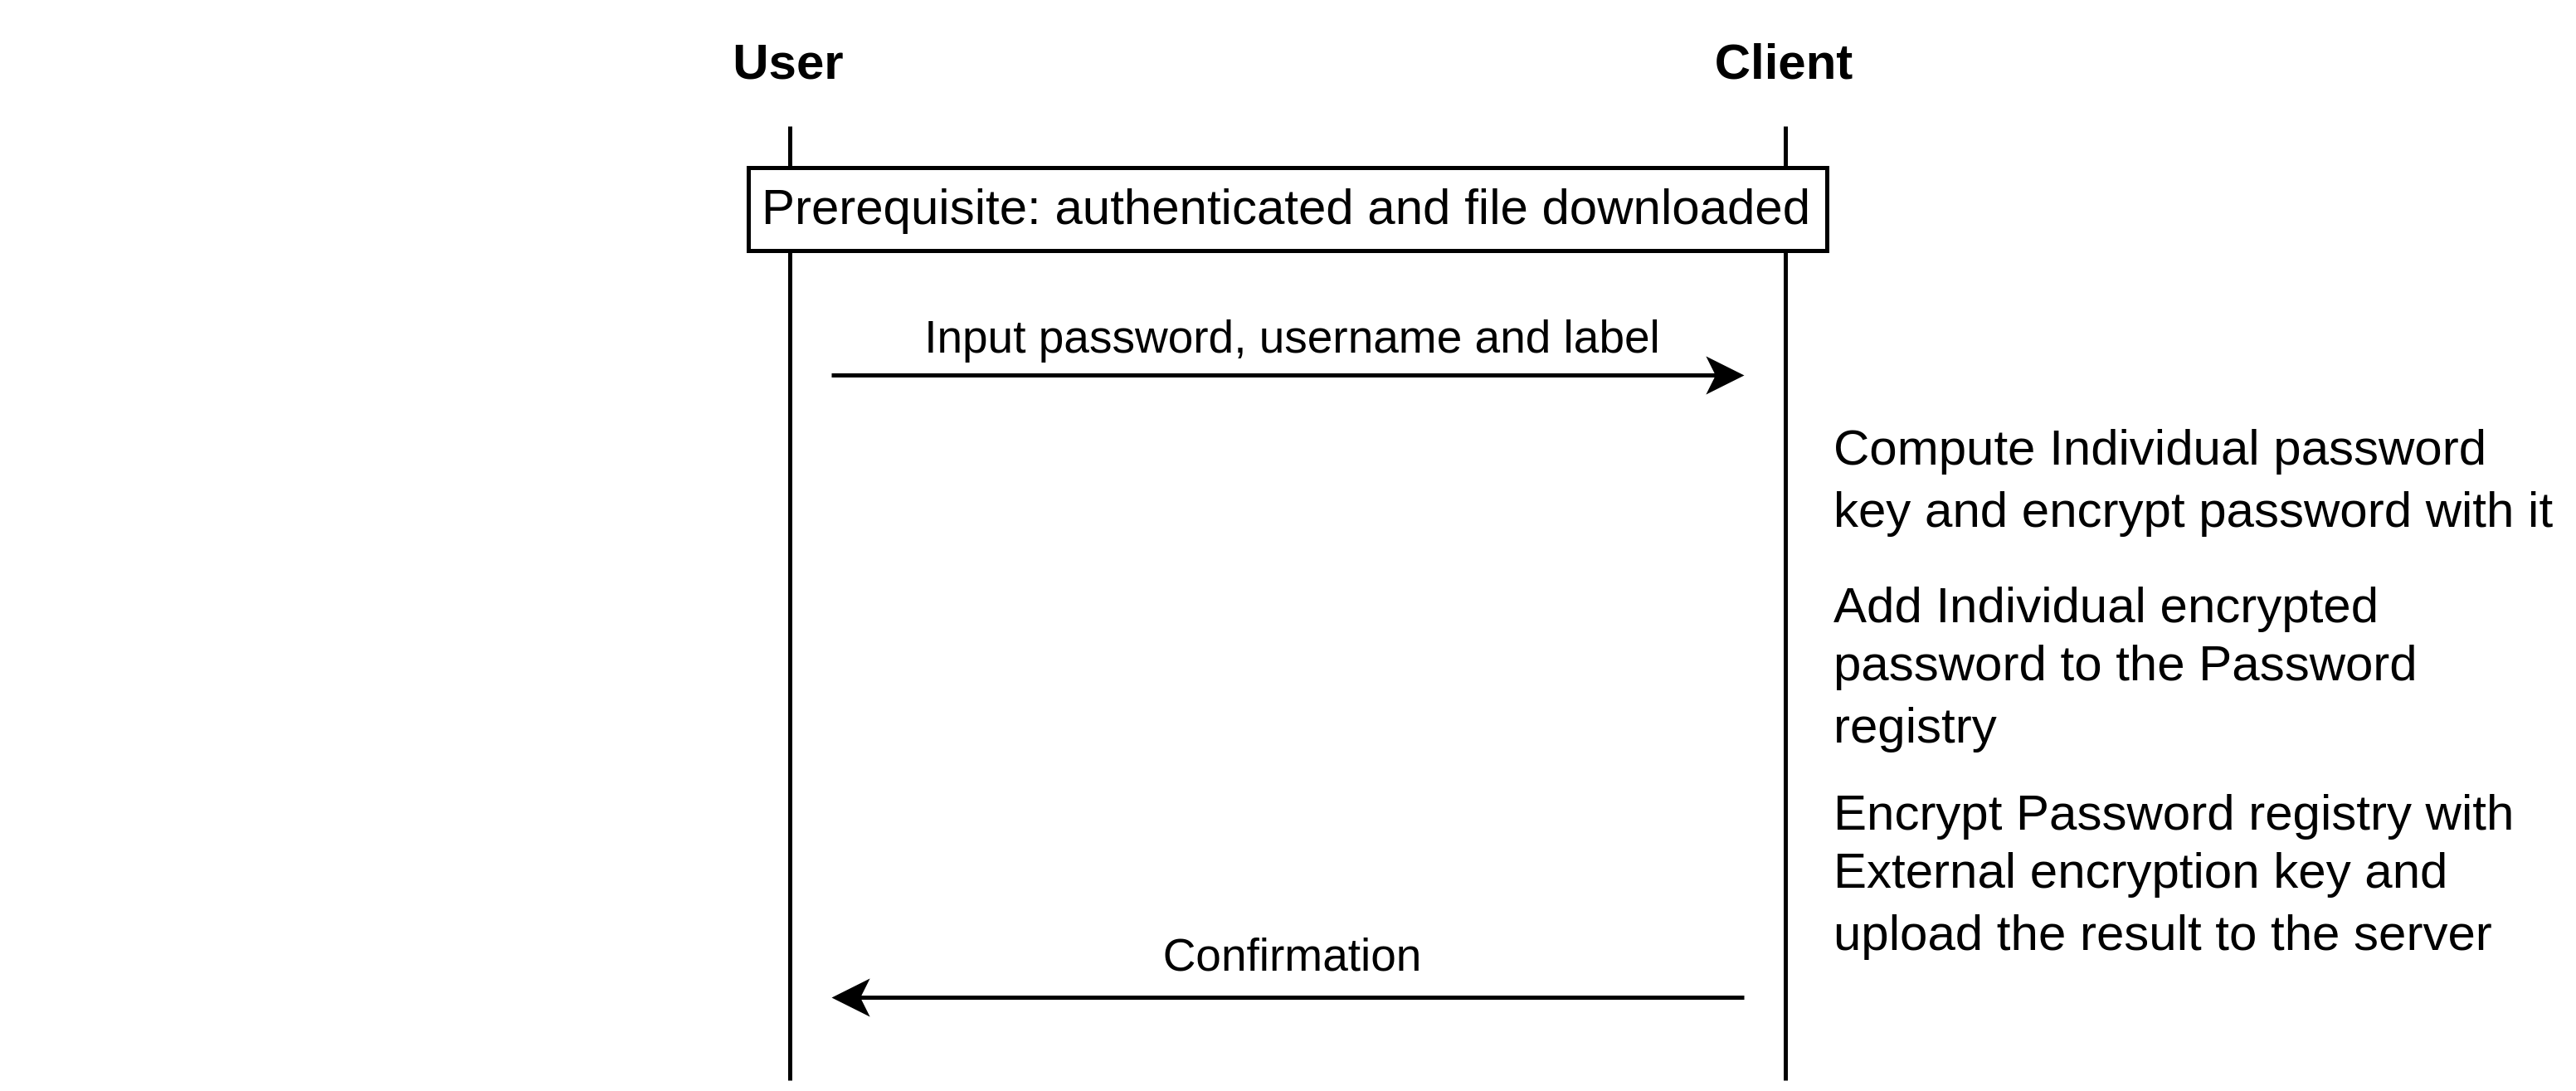
\includegraphics[width=\textwidth-22pt]{add.png}}

 \caption{Interaction between the user and the client for adding a new password entry.}
 \label{fig:usecase_add}
\end{figure}



\begin{figure}[h]
 \centering

 \setlength{\fboxsep}{10pt}
 \setlength{\fboxrule}{1pt}
 \fbox{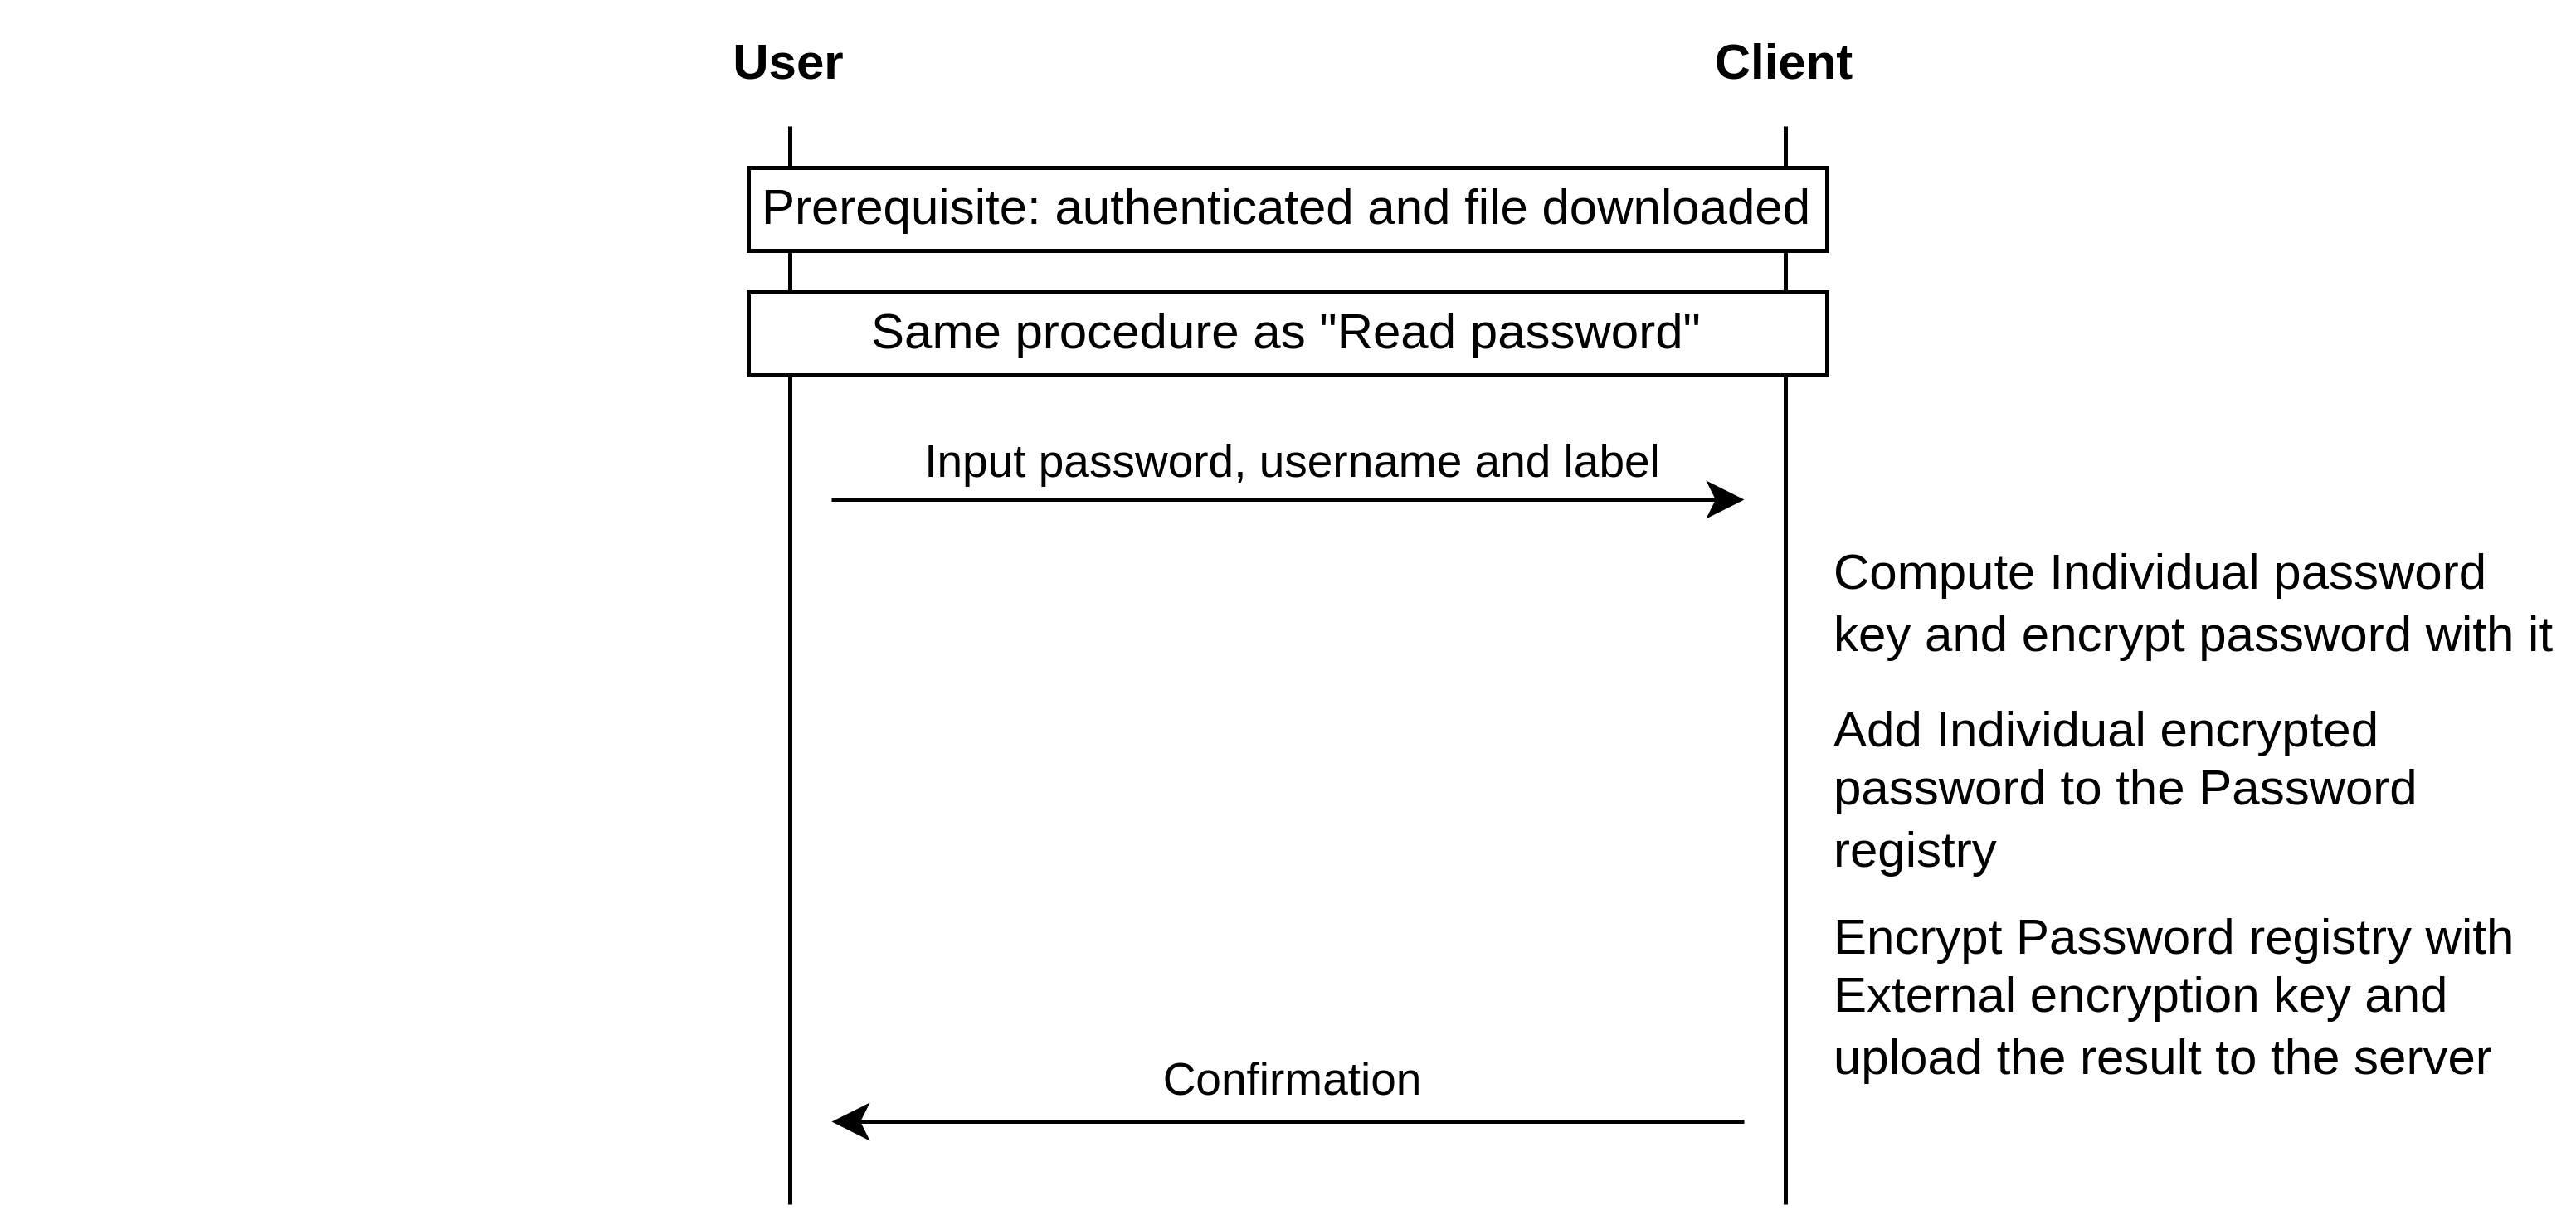
\includegraphics[width=\textwidth-22pt]{modify.png}}

 \caption{Interaction between the user and the client for modifying an existing password entry.}
 \label{fig:usecase_modify}
\end{figure}



\begin{figure}[h]
 \centering

 \setlength{\fboxsep}{10pt}
 \setlength{\fboxrule}{1pt}
 \fbox{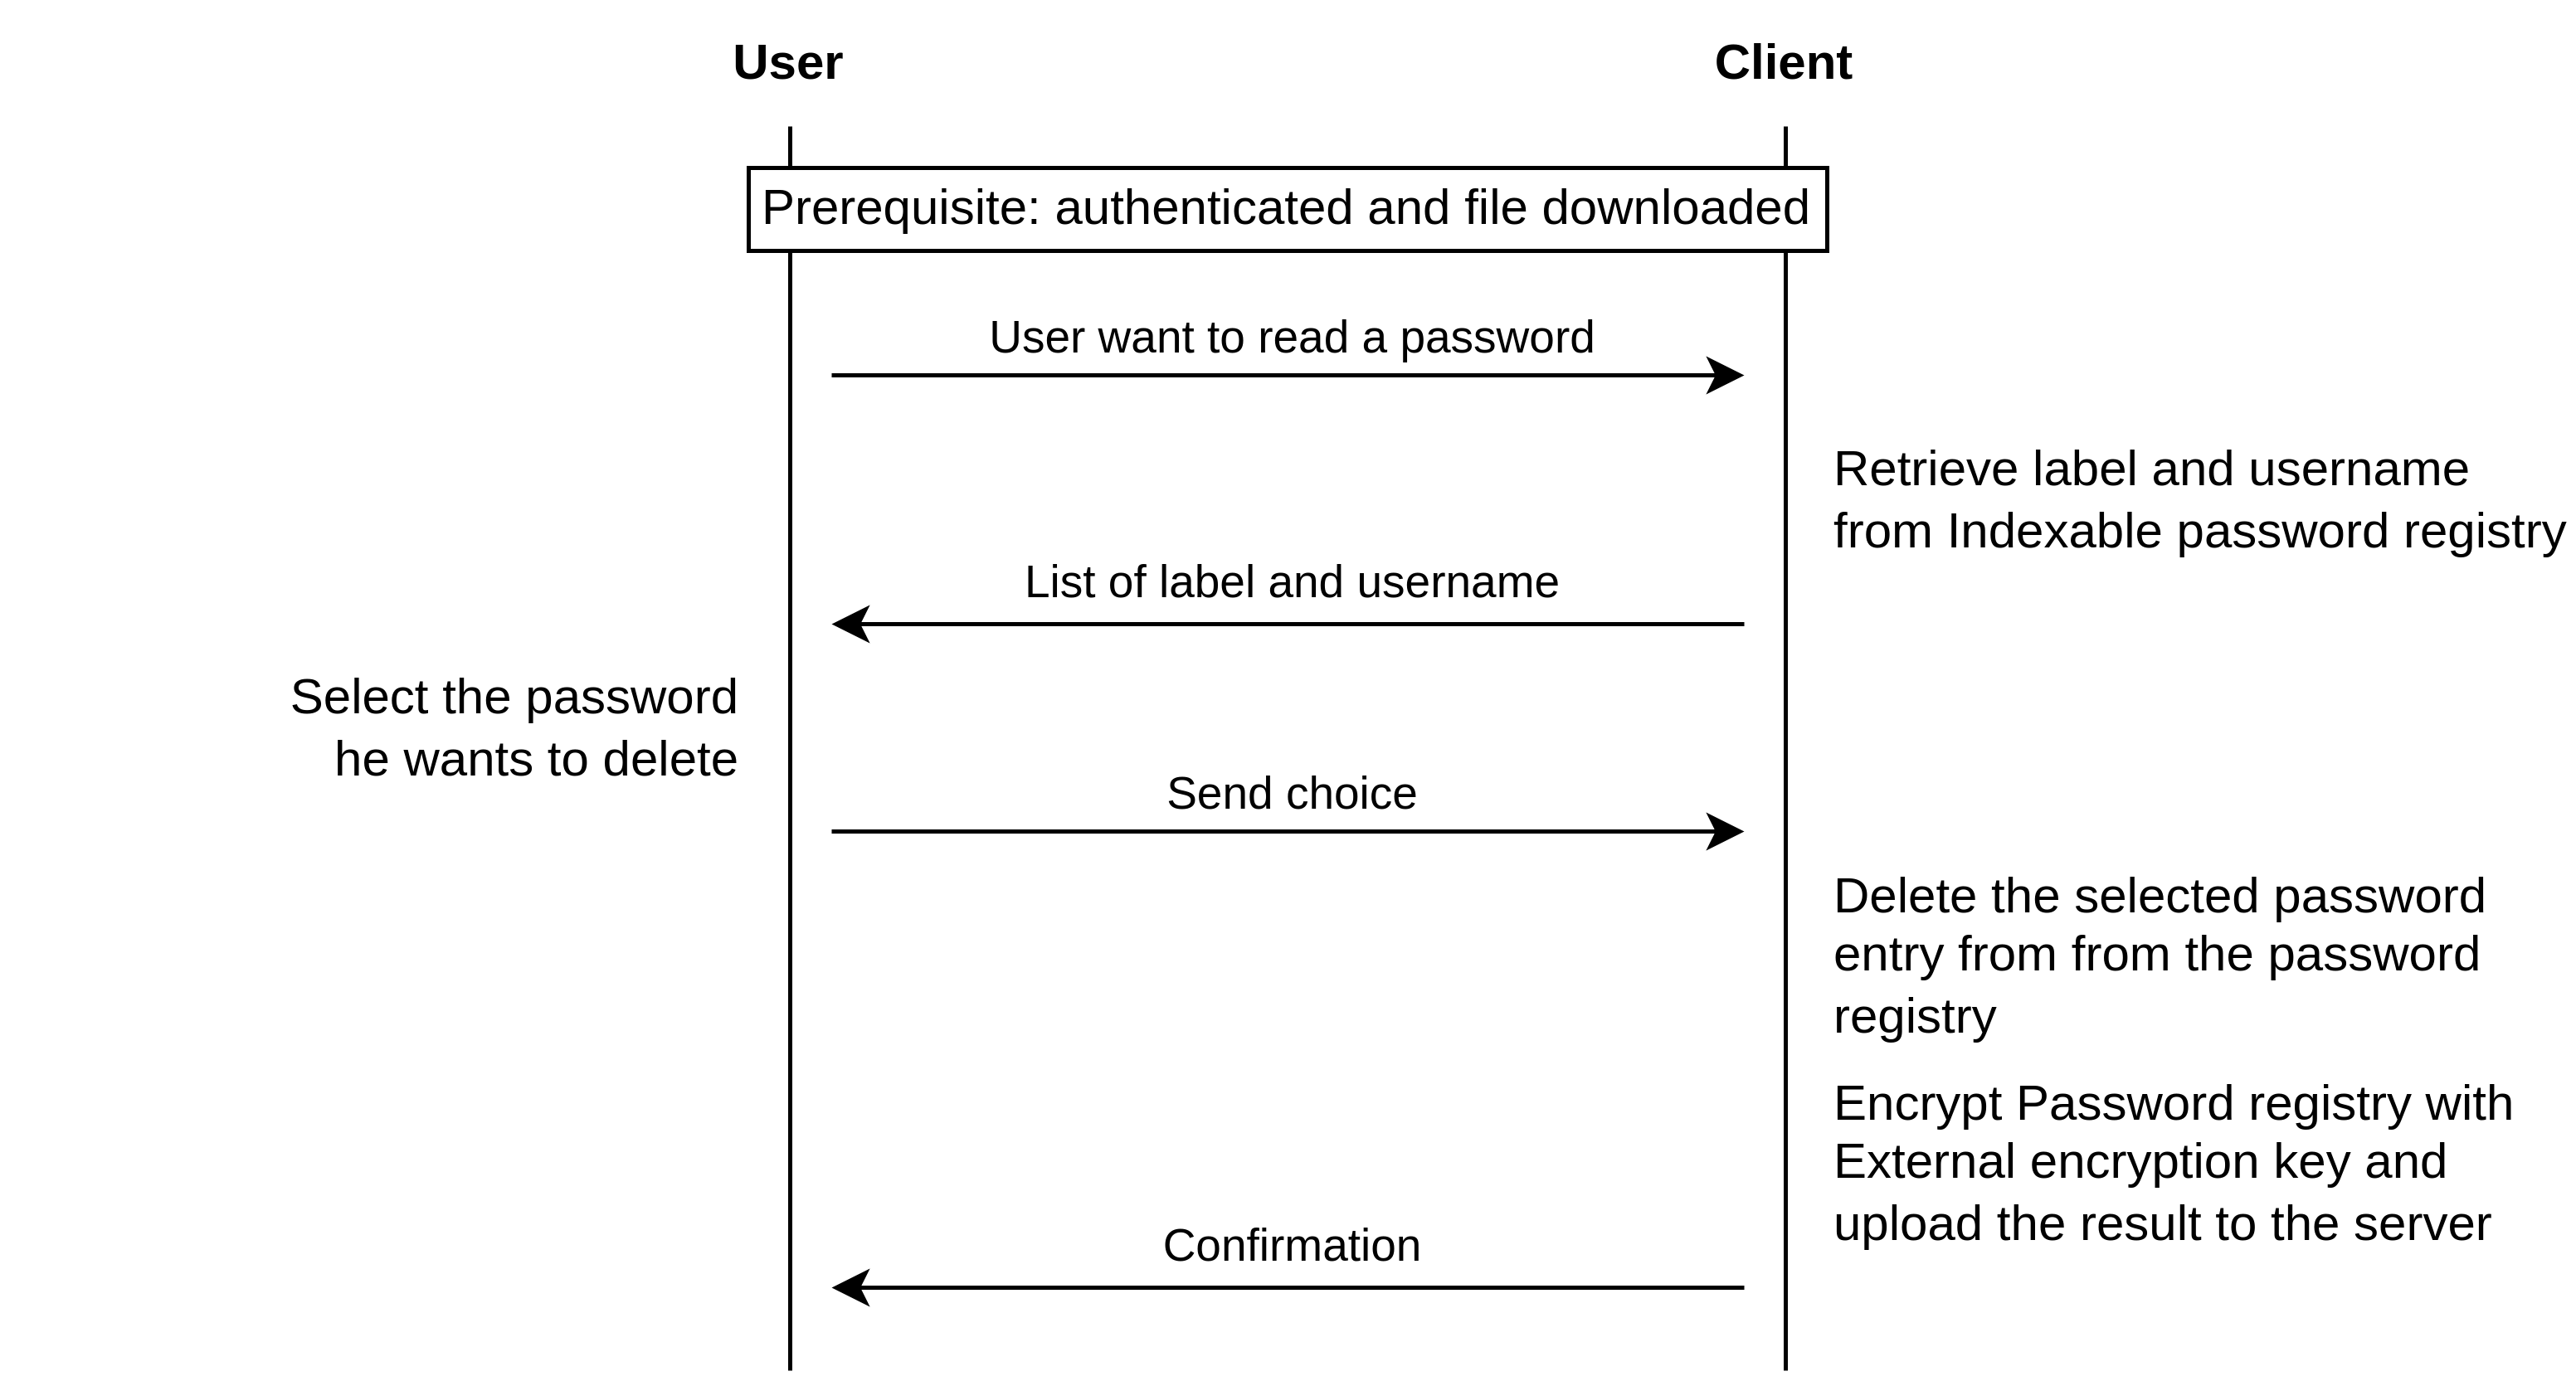
\includegraphics[width=\textwidth-22pt]{delete.png}}

 \caption{Interaction between the user and the client for deleting a password entry.}
 \label{fig:usecase_delete}
\end{figure}

\subsection{Advantages of KHAPE}
- no password on the server
- use of export key, an OPRF derived key. OPRF computation is more secure than deriving a key only on the client since an attacker will be forced to perform online guess (since he doesn't know OPRF secret salt). And avoid to recompute a slowhash on the password since it's already done in the KHAPE protocol

\subsection{Security considerations}
- in memory
- no implemented memory

\end{document}

